\documentclass[11pt, english]{article}
\usepackage{graphicx}
\usepackage[colorlinks=true, linkcolor=blue]{hyperref}
\usepackage[english]{babel}
\selectlanguage{english}
\usepackage[utf8]{inputenc}
\usepackage[svgnames]{xcolor}

\makeatletter
\renewcommand\paragraph{\@startsection{paragraph}{4}{\z@}%
            {-2.5ex\@plus -1ex \@minus -.25ex}%
            {1.25ex \@plus .25ex}%
            {\normalfont\normalsize\bfseries}}
\makeatother
\setcounter{secnumdepth}{4}
\setcounter{tocdepth}{4} 

\usepackage{listings}
\usepackage{afterpage}
\pagestyle{plain}

\definecolor{dkgreen}{rgb}{0,0.6,0}
\definecolor{gray}{rgb}{0.5,0.5,0.5}
\definecolor{mauve}{rgb}{0.58,0,0.82}

\usepackage{color, colortbl}
\definecolor{Gray}{gray}{0.9}
\definecolor{LightCyan}{rgb}{0,0,0}
\newcolumntype{g}{>{\columncolor{Gray}}c}

\newcommand*{\email}[1]{%
    \normalsize\href{mailto:#1}{#1}\par
}

\usepackage{hyperref}
\hypersetup{
    colorlinks=true,
    linkcolor=black,
    filecolor=blue,      
    urlcolor=black,
}

%\lstset{language=R,
%    basicstyle=\small\ttfamily,
%   stringstyle=\color{DarkGreen},
%    otherkeywords={0,1,2,3,4,5,6,7,8,9},
%    morekeywords={TRUE,FALSE},
%    deletekeywords={data,frame,length,as,character},
%    keywordstyle=\color{blue},
%    commentstyle=\color{DarkGreen},
%}

\lstset{frame=tb,
language=R,
aboveskip=3mm,
belowskip=3mm,
showstringspaces=false,
columns=flexible,
numbers=none,
keywordstyle=\color{blue},
numberstyle=\tiny\color{gray},
commentstyle=\color{dkgreen},
stringstyle=\color{mauve},
breaklines=true,
breakatwhitespace=true,
tabsize=3
}

\usepackage{here}


\textheight=21cm
\textwidth=17cm
%\topmargin=-1cm
\oddsidemargin=0cm
\parindent=0mm
\pagestyle{plain}

%%%%%%%%%%%%%%%%%%%%%%%%%%
% La siguiente instrucción pone el curso automáticamente%
%%%%%%%%%%%%%%%%%%%%%%%%%%

\usepackage{color}
\usepackage{ragged2e}

\global\let\date\relax
\newcounter{unomenos}
\setcounter{unomenos}{\number\year}
\addtocounter{unomenos}{-1}
\stepcounter{unomenos}
\gdef\@date{Year 2018 / 2019}

\begin{document}

\begin{titlepage}

\begin{center}
\vspace*{-1in}
\begin{figure}[htb]
\begin{center}

\includegraphics[width=8cm]{politoLogo.png}
\end{center}
\end{figure}

\begin{large}
\textbf{\underline{POLITECNICO DI TORINO}} \\
\end{large}
\vspace*{0.15in}
DISTRIBUTED PROGRAMMING 2 - \@date \\ 
\vspace*{0.4in}
\begin{large}
SPECIAL PROJECT 3 \\
\end{large}
\vspace*{0.2in}
\begin{Large}
\textbf{DATA MODELS FOR NFV ARCHITECTURES} \\
\end{Large}
\vspace*{0.3in}
\begin{large}
Enrico Cecchetti, \email{s253823@studenti.polito.it}
Federico Gianno, \email{s255548@studenti.polito.it} 
\end{large}
\vspace*{0.3in}
\rule{80mm}{0.1mm}\\
\vspace*{0.1in}
\begin{large}
Referrals: \\
Fulvio Valenza, \\
Jaloliddin Yusupov, \\
Riccardo Sisto \\
\end{large}
%\includegraphics[width=10cm]{LogoFac.jpg}
\end{center}
\end{titlepage}

\newcommand{\CC}{C\nolinebreak\hspace{-.05em}\raisebox{.4ex}{\tiny\bf +}\nolinebreak\hspace{-.10em}\raisebox{.4ex}{\tiny\bf +}}
\def\CC{{C\nolinebreak[4]\hspace{-.05em}\raisebox{.4ex}{\tiny\bf ++}}}

\tableofcontents
\newpage

\section{Introduction}
This paper is for the subject \textit{Distributed programming II}. The purpose of the project is to:
\begin{itemize}
    \item Design a data format (described by means of an XML schema) for the representation of all the most relevant information in the NFV and SDN contexts.
    \item Design and implement a RESTful web service that permits to store and retrieve the NFV/SDN information.
\end{itemize}

\section{Background}
NFV and SDN are emerging paradigms that allow to separate the network’s control logic from the underlying routers and switches introducing the ability to program the network. In the following paragraphs, is proposed a standard to manage these two architectures.

\subsection{NFV: Network Function Virtualization}
The main idea of NFV is the decoupling of physical network equipment from the functions that run on them. This means that a network function, such as a firewall, can be dispatched to a TSP (Telecommunication Service Providers) as an instance of plain software.

The VNFs may then be relocated and instantiated at different network locations without necessarily requiring the purchase and installation of new hardware \cite{nfv_architecture}.

\subsection{SDN: Software-Defined Networking}
SDN is a network paradigm that give a breath of fresh air on the nowadays architecture and that can revolution all the model we are using up to now. The aim of SDN is to provide open interfaces that enable the development of software that can control the connectivity provided by a set of network resources and the flow of network traffic though them, along with possible inspection and modification of traffic that may be performed in the network \cite{sdn_architecture}.

\section{Starting point}
We started from \textit{VerifOO \& Verigraph} NFV schema. First of all, we studied its model and compared it with the most successful standard: \textbf{ETSI} and \textbf{TOSCA}. After summarized the major difference between ETSI and VerifOO/Verigraph, we started to modify their structure in order to be as closer as possible to the standard.

In table \ref{tab:tab0} are listed the major difference between the two models. Also a resume schema is available \href{https://raw.githubusercontent.com/netgroup-polito/nfv-data-model/master/data-format/doc/VerifOO-Verigraph_resume.png?token=AYIltK1i1rPj3A9TCg0QdBJZRZjgzM3lks5ci86JwA\%3D\%3D}{\underline{here}}.

\begin{table}[!h]
    \centering
    \begin{tabular}{ m{2cm}|m{3cm}|m{4cm}|m{5cm} }
    \hline
    VerifOO Verigraph element & ETSI corresponding element & ESTI description & Compliant with the standard \\
    \hline
    \rowcolor{Gray}
    NFV & NSD & NSD consists of statics information elements used by NFV Orchestrator to instantiate a Network Service. & More or less. The purpose is the same but the level of abstraction is different. \\
    \hline
    Graphs & NSD: nfv\_dependency & It defines the sequence in which various nodes and links within a VNF should be instantiated by VNF orchestrator. & ETSI does not provide a specific configuration of that item. \\
    \hline
    \rowcolor{Gray}
    Constraints & NSD:vnfd & It describes a VNF in terms of deployment and operations behaviours requirements. & More or less. It has some matching elements with the standard. \\
    \hline
    Node constraints & NSD:vnfd:vdu & Information elements concerning the VDU (e.g. processor and memory requirements). & Yes, but the standard is more detailed. \\
    \hline
    \rowcolor{Gray}
    Link constraints & NSD:vld & It describes the basic topology of the connectivity between one or more VNFs, and other required parameters. & Yes, but with less parameters with the respect to the standard. \\
    \hline
    Property definition & - & - & No, but it's useful for VerifOO/Verigraph workflow. \\
    \hline
    \rowcolor{Gray}
    Hosts & - & - & No, the standard does not provide physical infrastructure implementation. \\
    \hline
    Connection & - & - & No (same reasons of above). \\
    \hline
    \rowcolor{Gray}
    Network Forwarding Path & NSD:vnffgd & The traffic flow through a VNFFGD is controlled by a Forwarding Path element. & Not so much. In the standard there are a lot of elements that here are missing. \\
    \hline
    Parsing string & - & - & No. \\
    \hline
    \end{tabular}
    \caption{VerifOO/Verigraph vs ETSI} \label{tab:tab0}
\end{table}

To summarize: \textit{VerifOO \& Verigraph} is not really compliant with the standard: there are some elements that are missing, other ones with different names and/or attribute, also similar structures sometimes they got additional functional and sometimes less.

\section{Model Design}
\textbf{Network Function Vitalization} (NFV) is an entity containing two main blocks:
\begin{itemize}
    \item The Physical Network Infrastructure (PNI)
    \item The list of the Network Services offered by the network (NS) 
\end{itemize}

This implementation is not described in the standard, it cares only about the Network Services without infer anything about the physical structure that will host them. 

Here, is proposed a different structure with the respect to the standard, because we think that it is worth to store those additional information (PNIs) to manage the allocation of the virtual functions in the physical machines and retrieve them in future.

\begin{table}[ht]
    \centering
    \begin{tabular}{c|c|c|m{7cm}}
    \hline
    Identifier & Type & Cardinality & Description \\
    \hline
    \rowcolor{Gray}
    pni & Element & 1 & Map of the physical network infrastructure. \\
    \hline
    ns & Element & 0...1 & List of Network Service Descriptor within the network. \\
    \hline
    \end{tabular}
    \caption{Network Function Vitalization} \label{tab:tab1}
\end{table}

Neither in the \emph{ETSI} standard and \emph{TOSCA} does exist a definition for the NFV. They both start from the NSD entity.

Since PNI is necessary to \emph{VerifOO \& Verigraph} has been decided to left the root element (NFV), like in the previous schema, with, in addition to the physical structure, has been defined a new structure containing the Network Services Descriptors (NSD).

The previous schema was composed by both PNI and NSD without a clear difference between them, in terms of attribute and functionality. 

To have an overview of the whole schema see \href{https://raw.githubusercontent.com/netgroup-polito/nfv-data-model/master/data-format/doc/NFV_model_final.png?token=AYIltFsv8LRFrn_5Q9PjAYBe2HxRzoBFks5ci87twA\%3D\%3D}{\underline{this}}.

\subsection{PNI: Physical Network Infrastructure}
Entity containing the set of subnets within the network, its hosts and the relative connections between them.

\begin{table}[ht]
    \centering
    \begin{tabular}{c|c|c|m{7cm}}
    \hline
    Identifier & Type & Cardinality & Description \\
    \hline
    \rowcolor{Gray}
    hosts & Element & 0...N & Hosts which is part of the physical connections. \\
    \hline
    connections & Element & 0...N & Map of the physical connection within the network. \\
    \hline
    \end{tabular}
    \caption{NFV:PNI} \label{tab:tab2}
\end{table}

The whole block contains \emph{Hosts} and \emph{connections} has been moved inside this new entity called \textbf{PNI} in order to wrap them together.  

We decided to left this block outside the NS because the Physical Network Infrastructure does not concern the description of a Network Service. Then, it should not be included in the NS. This permits also to generalize the schema to make it compatible with wide range of tools.

Moreover, this approach allow us to implement a NS in such way that a future implementation will not require critical changes in the model.

\subsubsection{Hosts}
A branch (subnet) of the network infrastructure. 

\begin{table}[ht]
    \centering
    \begin{tabular}{c|c|c|m{7cm}}
    \hline
    Identifier & Type & Cardinality & Description \\
    \hline
    \rowcolor{Gray}
    host & Element & 1...N & Physical machine present in the network infrastructure. \\
    \hline
    \end{tabular}
    \caption{NFV:PNI:hosts} \label{tab:tab3}
\end{table}

The previous schema, adopted in \emph{VerifOO \& Verigraph}, has been maintained  because it is not a bad structure considering the lack of standard design.

\paragraph{Host}

\begin{table}[ht]
    \centering
    \begin{tabular}{c|c|c|m{7cm}}
    \hline
    \rowcolor{white}
    Identifier & Type & Cardinality & Description \\
    \hline
    \rowcolor{Gray}
    id & Attribute & 1 & ID of the physical machine. \\
    \hline
    \rowcolor{white}
    name & Attribute & 0...1 & Name of the physical machine. \\
    \hline
    \rowcolor{Gray}
    fixedEndPoint & Attribute & 0...1 & - \\
    \hline
    \rowcolor{white}
    active & Attribute & 1 & True if at least one node has been deployed on the host. \\
    \hline
    \rowcolor{Gray}
    maxVNF & Attribute & 1 & Maximum of Virtual Network Function that the host can handle. \\
    \hline
    \rowcolor{white}
    type & Element & 0...N & Defines the type of the host (e.g. client, server, middle-box). \\
    \hline
    \rowcolor{Gray}
    computational\_properties & Element & 0...1 & Describes the memory and cpu resources characteristics (e.g. cpu, cores, number of operations). \\
    \hline
    \rowcolor{white}
    memory\_properties & Element & 0...1 & Represents the physical memory of the host (e.g. memory, disk storage, virtual memory resources). \\
    \hline
    \rowcolor{Gray}
    network\_properties & Element & 0...1 & It represents the network characteristics (e.g. bandwidth). \\
    \hline
    \rowcolor{white}
    v\_node\_ref & Reference & 0...N & Reference to a virtual network function. \\
    \hline
    \rowcolor{Gray}
    p\_node\_ref & Reference & 0...1 & Reference to a physical network function. \\
    \hline
    \rowcolor{white}
    supported\_VNF & Element & 0...N & Functional types which the host supports. \\
    \hline
    \end{tabular}
    \caption{NFV:PNI:hosts:host} \label{tab:tab4}
\end{table}

The main structure, more or less, remained the same. Some attributes has been grouped based on their purpose (e.g. computational properties: cpu, cores, number of operations, etc.). 

Also, has been added a physical node reference in order to connect to the network some physical devices that are not virtualized yet.

\subsubsection{Connections}
Map of the physical \textbf{connection}.

\begin{table}[ht]
    \centering
    \begin{tabular}{c|c|c|m{7cm}}
    \hline
    Identifier & Type & Cardinality & Description \\
    \hline
    \rowcolor{Gray}
    connection & Element & 0...1 & The connection between two or more hosts in terms of source, destination and latency. \\
    \hline
    \end{tabular}
    \caption{NFV:PNI:connections} \label{tab:tab5}
\end{table}

The previous schema, adopted in \emph{VerifOO \& Verigraph}, has been maintained  because it is not a bad structure considering the lack of standard design.

\subsection{NSD: Network Service Descriptor}
The NS is composed by a sequence of \textbf{NSD}: the Network Service Descriptor is a deployment template for a Network Service refereeing all other descriptors which describe components that are part of that network service.

\begin{table}[ht]
    \centering
    \begin{tabular}{c|c|c|m{7cm}}
    \hline
    Identifier & Type & Cardinality & Description \\
    \hline
    \rowcolor{Gray}
    id & Attribute & 1 & ID of this Network Service Descriptor. \\
    \hline
    vendor & Attribute & 0...1 & Provider or Vendor of this Network Service. \\
    \hline
    \rowcolor{Gray}
    version & Attribute & 0...1 & Version of the Network Service Descriptor. \\
    \hline
    vnf\_dependency & Element & 0...1 & Describes dependencies between VNF. \\
    \hline
    \rowcolor{Gray}
    property\_definition & Element & 0...1 & List of properties that will be checked by VerifOO for a specific graph (useful for VerifOO and Verigraph). \\
    \hline
    vnf & Element & 0...1 & VNF which is part of the Network Service. \\
    \hline
    \rowcolor{Gray}
    vnffgd & Element & 0...1 & VNFFGD which is part of the Network Service. \\
    \hline
    pnf & Element & 0...1 & PNFs which are part of the Network Service. \\
    \hline
    \rowcolor{Gray}
    flavours & Element & 0...1 & Represent the service KPI parameters and its requirement for each deployment flavors of the NS being described. For example flavour describing the requirement for support a service with 300k calls per second.  \\
    \hline
    connetion\_points & Element & 0...1 & List of connection points which acts as an end point of the Network Service. \\
    \hline
    \end{tabular}
    \caption{NFV:NS:NSD} \label{tab:tab6}
\end{table}

\textbf{NSD} has been designed has much as possible closer to the standard. 

Has been inserted some different entities with the respect to the previous \emph{VerifOO \& Verigraph} schema because it was not very compliant with the standard. For the same reason, the name of other elements has been modified with the corresponding ETSI's name.

These elements has been added: id, vendor, version, pnfd, service\_deployment\_flavour and connection point.

Instead, these elements has been modified:
\begin{itemize}
    \item Graphs $\rightarrow$ nfv\_dependencies
    \item Constraints $\rightarrow$ vnfd
    \item Network Forwarding Path $\rightarrow$ vnffgd
\end{itemize}

\subsubsection{VNF Dependency}
Describe dependencies between VNF. Defined in terms of source and target VNF, i.e. target VNF "depends on" source VNF. In other words a source VNF shall exist and connect to the service before target VNF can be initiated/deployed and connected. This element would be used, for example, to define the sequence in which various numbered network nodes and links within a VNFFGD should be instantiated by the NFV Orchestrator.

\begin{center}
    \begin{figure}[h!]
        \centering
        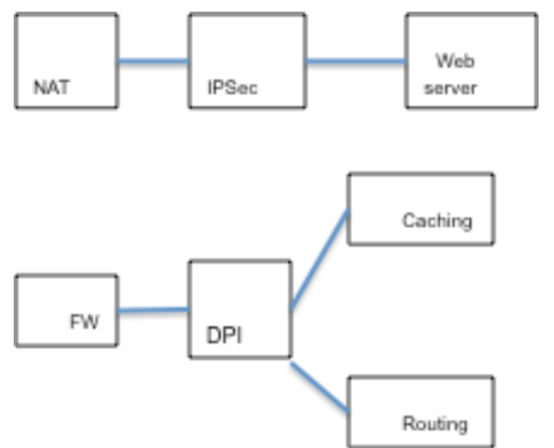
\includegraphics[width=9cm, height=5cm]{vnf_dependency.png}
        \caption{Network composed by two subnets, respectively with 3 and 4 hosts.} \label{Fig1}
    \end{figure}
\end{center}

The ETSI standard does not provide a specific schema for this element. Therefore, has been decided to not change the main structure proposed by \emph{VerifOO \& Verigraph} schema. To be exactly the same as the standard, \textit{graphs} has been renamed as \textbf{vnf\_dependecy}. Also an attribute has been added: \textit{vnfd\_id}, that is a referenced by the \textit{id} of VNFD and it is indicating what kind of VNF that node is providing. See \cite{etsi}, clause 6.2.1.1.

\newpage
\subsubsection{Property Definition}
\textbf{Property Definition} is not defined neither in ETSI neither in TOSCA. Has been decided to leave it in order to not compromise the correct functionality of \emph{VerifOO \& Verigraph}.

\subsubsection{VNFD: Virtual Network Function Descriptor}
VNF is a sequence of \textbf{VNFD}, a deployment template which describes a VNF in terms of its deployment and operational behavior requirements. The information provided in the VNFD should be used by an Orchestrator to manage and orchestrate Network Services and virtualized resources.

\begin{table}[ht]
    \centering
    \begin{tabular}{c|c|c|m{7cm}}
    \hline
    Identifier & Type & Cardinality & Description \\
    \hline
    \rowcolor{Gray}
    id & Attribute & 1 & ID for this Virtual Network Function Descriptor. \\
    \hline
    vendor & Attribute & 0...1 & Provider or Vendor of this Virtual Network Function. \\
    \hline
    \rowcolor{Gray}
    version & Attribute & 0...1 & Version of the Virtual Network Function Descriptor. \\
    \hline
    vdu & Element & 1...N & Describes a set of elements related to a particular VDU. \\
    \hline
    \rowcolor{Gray}
    virtual\_link & Element & 0...N & Describes the required parameters. The name has been changed from the previous ‘connections’. \\
    \hline
    dependency & Element & 0...N & Dependencies between VDUs. Defined in terms of source and target VDU. \\
    \hline
    \end{tabular}
    \caption{NFV:NSD:vnf:vnfd} \label{tab:tab7}
\end{table}

In the previous model, the \textbf{VNFD} entity was ambiguous: it was called with another name (constraints). 
Its elements \textit{LinkConstraints} and \textit{NodeConstraints}, the actual \textbf{vdu} and \textbf{virtual\_link}, were incomplete and messy. This is due to the fact that the properties was massed all inside to a single entity.

Has been introduced one new entity: \textit{dependency}, present in the standard. Motivation will be reported in the corresponding section. 

\newpage
\paragraph{VDU: Virtual Deployment Unit}
The \textbf{VDU} is a basic part of VNF. It is the VM that hosts the network functions. It describes the properties like \emph{image} to be used in VDU, \emph{management driver} to be used, \emph{flavour} describing physical properties for the VDU to be spawned, etc.

\begin{table}[ht]
    \centering
    \begin{tabular}{c|c|c|m{7cm}}
    \hline
    Identifier & Type & Cardinality & Description \\
    \hline
    \rowcolor{Gray}
    id & Attribute & 1 & ID of this Virtual Deployment Unit. \\
    \hline
    vm\_image & Attribute & 0...1 & Provides a short description of the VM. \\
    \hline
    \rowcolor{Gray}
    computation\_requirements & Element & 1 &  Describes the memory and cpu resources characteristics (e.g. cpu, cores, number of operations). \\
    \hline
    memory\_requirements & Element & 0...1 &  Describes the memory and cpu resources characteristics (e.g. cpu, cores, number of operations). \\
    \hline
    \rowcolor{Gray}
    network\_requirements & Element & 0...1 &  Represents the network requirements (e.g. bandwidth). \\
    \hline
    \end{tabular}
    \caption{NFV:NS:NSD:vnf:vnfd:vdu} \label{tab:tab8}
\end{table}

First of all, has been added the attribute \textbf{vm\_image}, that is a generic description about the  characteristic of the virtual machine. It is implemented by both ETSI and TOSCA. However, it has been designed as a generic string because ETSI standard does not provide a specific implementation about the VM information, instead TOSCA propose a very detailed structure about that.

More details about TOSCA VM at \cite{tosca}, see clause 5.4.1.1.

Then, regarding the other changes, \textit{metrics} has been split into three different blocks, each one specific for a requirement type: \textbf{computation\_requirements}, \textbf{memory\_requirements} and \textbf{network\_requirements}. The split is due to the fact that these requirements was all inside the same entity but without a distinction between them. Moreover, this approach will permit future implementation and it is better compliant with the standard.

See \cite{etsi} clause 6.3.1.2.

\newpage
\paragraph{Virtual Link}
\textbf{Virtual link} is a deployment template which describes the resources requirement that are needed for a link between VNFs, PNFs and end-point of the Network Service.

\begin{table}[ht]
    \centering
    \begin{tabular}{c|c|c|m{7cm}}
    \hline
    Identifier & Type & Cardinality & Description \\
    \hline
    \rowcolor{Gray}
    src & Attribute & 1 & Source connection point of a VNF. \\
    \hline
    dst & Attribute & 1 & Destination connection point of a VNF. \\
    \hline
    \rowcolor{Gray}
    test\_access & Attribute & 0...1 & Describes test access facilities to be supported on the VL (e.g. none, passive, monitoring or active (intrusive) loopbacks at endpoints). \\
    \hline
    qos & Element & 0...N &  Describes Quality of Service options to be supported on virtual link (e.g latency, jitter). \\
    \hline
    \end{tabular}
    \caption{NFV:NS:NSD:vnf:vnfd:virtual\_link} \label{tab:tab9}
\end{table}

The structure is more ore less similar to the previous one. The attribute \emph{requiredLatency} has been included inside the new entity \textbf{qos} (Quality of Service). The creation of this element permits to include inside a single entity, not only the latency, but also other related parameters. In this way the model is more similar to the standard and is possible to store other data (as the \textit{jitter}) that are cited by ETSI.

See \cite{etsi}, clause 6.3.1.3.

Like in TOSCA and ETSI, has been introduced the \textbf{test\_access} entity. It passively/actively can  capture traffic on a network and use it to monitor the network traffic between two points of the network.

See \cite{etsi}, clause 6.3.1.3; or \cite{tosca}, clause 5.9.6.1.

\paragraph{Dependency}
This a new entity, that represents the constraint in terms of target VDU "depends on" source VDU. In other words, sources VDU shall exists before target VDU can be initiated/deployed. 

Speaking about the \textit{xsd} schema, the element \textbf{dependency} is a sequence of elements \emph{relations}, each one composed by two references to a source VDU and destination VDU.

See \cite{etsi}, clause 6.3.1.1.

\newpage
\subsubsection{VNFFGD: VNF Forwarding Graph Descriptor}
\textbf{VNFFGD} is a deployment template which describes a topology of the network service or a portion of the network service by referencing VNFs and PNFs and Virtual Links that connect them.

\begin{table}[ht]
    \centering
    \begin{tabular}{c|c|c|m{7cm}}
    \hline
    Identifier & Type & Cardinality & Description \\
    \hline
    \rowcolor{Gray}
    id & Attribute & 0...1 & ID for the VNFFG Descriptor. \\
    \hline
    vnffgd\_security & Attribute & 0...1 & This is a signature of vnffgd to prevent tampering. The particular hash algorithm used to compute the signature, together with the corresponding cryptographic certificate to validate the signature should also be included. \\
    \hline
    \rowcolor{Gray}
    network\_forwarding\_path & Element & 0...N & Describes a network forwarding graph within the VNFFGD. \\
    \hline
    \end{tabular}
    \caption{VNF:NS:NSD:vnffgd} \label{tab:tab10}
\end{table}

The main structure is, more or less, the same as \emph{VerifOO \& Verigraph}. Some elements has been renamed: from \textit{Network Forwarding Path} to \textbf{vnffgd} and from \textit{path} to \textbf{network\_forwarding\_path}. A new entity has been added \textbf{vnffgd\_security}, it contains the policy to assure the security of the forwarding path.

See \cite{etsi}, clause 6.5.1.1.

\paragraph{Network forwarding path}

\begin{table}[ht]
    \centering
    \begin{tabular}{c|c|c|m{7cm}}
    \hline
    Identifier & Type & Cardinality & Description \\
    \hline
    \rowcolor{Gray}
    id & Attribute & 1 & Specify the identifier (e.g. name) of the Network Forwarding Path. \\
    \hline
    n\_endpoint & Attribute & 0...1 & Count of the external endpoints included in this VNFFG, to form an index. \\
    \hline
    \rowcolor{Gray}
    n\_vl & Attribute & 0...1 & Count of the VLs used by this VNFFG, to form an index. \\
    \hline
    connection & Element & 2...N & Reference to a Connection Point forming the VNFFG. \\
    \hline
    \end{tabular}
    \caption{VNF:NS:NSD:vnffgd:netork\_forwarding\_path} \label{tab:tab11}
\end{table}

In this section has been added some information that could be useful for some kind of analysis (\textbf{n\_endpoint} and \textbf{n\_vl} indexes).
Also, the name of \textit{path Node} has been changed to \textbf{connection}, as the standard. 

See \cite{etsi}, clause 6.5.1.1 \& 6.5.1.2.

\subsubsection{PNFD: Physical Network Function Descriptor}
PNF is a list of\textbf{Physical Network Function Descriptor} (PNFD) that describes the connectivity, Interface and KPIs requirements of Virtual Links to an attached Physical Network Function. This is needed if a physical device is incorporated in a Network Service to facilitate network evolution \cite{etsi}.

\begin{table}[ht]
    \centering
    \begin{tabular}{c|c|c|m{7cm}}
    \hline
    Identifier & Type & Cardinality & Description \\
    \hline
    \rowcolor{Gray}
    id & Attribute & 1 & The ID (e.g. name) of this PNFD. \\
    \hline
    vendor & Attribute & 0...1 & The vendor generating this PNFD. \\
    \hline
    \rowcolor{Gray}
    version & Attribute & 0...1 & The version of PNF this PNFD is describing. \\
    \hline
    description & Attribute & 0...1 &  This element describes an external interface exposed by this PNF enabling connection with a VL. \\
    \hline
    \rowcolor{Gray}
    connection\_point & Element & 0...1 & Physical connection point of the PNFD. \\
    \hline
    \end{tabular}
    \caption{VNF:NS:NSD:pnf:pnfd} \label{tab:tab12}
\end{table}

Has been decided to introduced this new element because it is expected by the standard (see \cite{etsi}, clause 6.6.1). As written in \cite{pnfd}, many service providers have made huge investments in these appliance based solutions and quite rightly expect to continue to realize the benefit of these investments for some years into the future.

\paragraph{Connection point}
The following table represents the structure of the \textbf{connection\_point} previously cited.

\begin{table}[ht]
    \centering
    \begin{tabular}{c|c|c|m{7cm}}
    \hline
    Identifier & Type & Cardinality & Description \\
    \hline
    \rowcolor{Gray}
    id & Attribute & 1 & ID of the Connection Point \\
    \hline
    type & Attribute & 0...1 & This may be for example a virtual port, a virtual NIC address, a physical port, a physical NIC address or the endpoint of an IP VPN enabling network connectivity. \\
    \hline
    \end{tabular}
    \caption{NFV:NS:NSD:pnf:pnfd:connection\_point} \label{tab:tab13}
\end{table}

\subsubsection{Service Deployment Flavour}
TOSCA and ETSI provide two different implementation for the \textbf{Deployment Flavour}:
\begin{itemize}
    \item TOSCA inserts the flavour only inside the Virtual Link Descriptor: it describes a specific flavour of the VL with specific bit-rate requirements.
    
    See \cite{tosca}, clause 5.9.6.1.
    \item ETSI propose two different flavour:
        \begin{itemize}
            \item One inside the VNFD, in order to represent the assurance parameters and its requirements for each deployment flavours being descripted (e.g. 10k call per second).
            
            See \cite{etsi}, clause 6.3.1.5.
            
            \item One in the NSD, that is the proposed one. It represents the assurance parameters of the Network Service being descripted.
            
            See \cite{etsi}, clause 6.2.1.3.
        \end{itemize}
\end{itemize}

\begin{table}[ht]
    \centering
    \begin{tabular}{c|c|c|m{7cm}}
    \hline
    Identifier & Type & Cardinality & Description \\
    \hline
    \rowcolor{Gray}
    id & Attribute & 1 & ID of the deployment flavour. \\
    \hline
    flavour\_key & Attribute & 1 & Assurance parameter against which this flavour is being described. For example, a flavour of a virtual EPC could be described in terms of the assurance parameter "calls per second" (cps).\\
    \hline
    \rowcolor{Gray}
    flavour\_value & Attribute & 1 & Value associated to the flavour\_key. \\
    \hline
    \end{tabular}
    \caption{NFV:NS:NSD:flavours:service\_deployment\_flavour} \label{tab:tab14}
\end{table}

Flavours are constraints about a certain service or function (e.g. 1k calls per second) that must be assured.  ETSI propose two levels of flavour: service\_deployment\_flavour (inside the NSD) and deployment\_flavour (inside VNFD).

The flavours contain the constraints and the reference to the VNFs (if NDS's flavour) or VDUs (otherwise) that permits to ensure that.

The idea is that the flavor inside the VNFD could be avoided because it is too hard to design and it carries useless information. Instead, has been implemented the \textit{flavour} of the NSD because it could be useful for future implementation. Right now, it may not be used but in this way the model represents a good starting point for future implementations.

\subsubsection{Connection Point}
Connection points contains the sequence of \textbf{Connection point} that represents a possible connection point of that Network Service.

\begin{table}[ht]
    \centering
    \begin{tabular}{c|c|c|m{7cm}}
    \hline
    Identifier & Type & Cardinality & Description \\
    \hline
    \rowcolor{Gray}
    id & Attribute & 1 & ID of the Connection Point. \\
    \hline
    type & Attribute & 1 & This may be for example a virtual port, a virtual NIC address, a physical port, a physical NIC address or the endpoint of an IP VPN enabling network connectivity. \\
    \hline
    \end{tabular}
    \caption{NFV:NS:NSD:connectio\_points:connection\_point} \label{tab:tab15}
\end{table}

This element has been added because it is provided by ETSI. In the future it could be exploited by connecting different Network Service between them. It may be used in a Software Developed Network.

See \cite{etsi}, clause 6.2.1.2.

\section{RESTful web service}
The developed \textbf{RESTful web service} allows to store and retrieve information about the NFV schema previously described. It permits to add, delete and modify not only the entire structure of the network but also its sub-parts.

\subsection{Development}
The RESTful has been developed both in Eclipse Neon 2 and IntelliJ IDEA, with the following features:
\begin{itemize}
    \item Framework: Jersey 2.2 and JAXB
    \item Server: Tomcat v8.5 (for Eclipse) and Glassfish 4.1 (for IntelliJ)
    \item Swagger API
\end{itemize}

The used library are available  \href{https://github.com/netgroup-polito/nfv-data-model/tree/master/lib}{\underline{here}}.

In the \href{https://github.com/netgroup-polito/nfv-data-model/blob/master/README.md#configuration}{\underline{GitHub repo}} is described how to configure the environment for both \textit{Eclipse} and \textit{IntelliJ IDEA}. It is also available the \href{https://github.com/netgroup-polito/nfv-data-model}{\underline{source code}}. 

\subsection{Granularity}
First of all, it is possible to GET, POST and DELETE the root element \textbf{NFV} and also the sub-root \textbf{PNI} and \textbf{NS}. Notice that, for these elements, the POST will overwrite all the previous structures (if there was one). This choice is due to the fact that in PNI, for example, if you want to add more \textit{Host} or \textit{Connection}, you can just use the relative Method instead of POST from the root. For the same reason, this approach has been adopted both in NFV and in NS.

Focusing on the sub-structures of PNI, it is allowed GET, POST, DELETE and also PUT (MODIFY) a single or multiple \textbf{Hosts} and/or \textbf{Connections}. In this way is very easy to modify the Physical Network Structure. It is not allowed to perform operations on the attributes and/or elements of \textit{Host} and \textit{Connection}: if you want to perform some kind of operations in that attributes/elements just perform it on the Host/Connection. The motivation is that the properties of a certain host will hardly change if the hosts itself will not change. So, at that point, if a specific requirements need to be changed probably also the host would need a change. Therefore, no methods to GET, POST and DELETE elements of Host and Connection. 

Regarding \textbf{NSD}, it is possible to GET, POST and DELETE a NSD, but is not allowed to PUT (MODIFY) an existing NSD: if you want to modify a certain NSD just use the relative method that will allow you to modify each single element of that NSD.

About \textbf{VNFDependency}, same considerations of NSD can be done. Moreover, a POST of VNFDepdency will overwrite all the previous structures. If you want to add something just use the relative method for that element. In this way, for example, if you want to add multiple \textit{graph}, for each graph a response will be provided with a feedback related to the used method. Adding more than one graph contemporaneously, it will not possible to have a response for each graph but it will only possible to have a global response. So, if one graph could not be added to the structure it will not reported because, maybe, the other \textit{n} graph will be added correctly. By adding one graph at time it will be possible to have more control on what is happening within the system.

Concerning its elements, \textbf{Graph} and \textbf{Node}, it is possible to GET, POST and DELETE but not  to PUT (MODIFY) a graph. If you want to modify a graph, for sure you need to add, remove or modify some nodes of that graph, so just use the relative method of node that will allow you to POST, DELETE and PUT (MODIFY) a node. If you need to modify the \textit{neighbour} or a \textit{configuration} of a certain node just modify the node. Same motivations of host can be done.

For \textbf{PropertyDefinition}, the methods will allow you to GET, POST and DELETE all the defined \textit{property}: for the same reason of VNFDependency, if you POST a \textit{ProeprtyDefinition} it will overwrite all the previous structures. Just use the relative methods of \textbf{Property} that will allow you to GET, POST, DELETE and PUT (MODIFY) a single property.

The same considerations of VNFDependency can be done for \textbf{VNF}. So, it is permitteed to GET, POST and DELETE of a VNF and the POST will overwrite the previous structures.

Concerning its elements, it is only allowed to GET, POST, DELETE and PUT (MODIFY) the \textbf{VNFD}. It is not permitted to perform operations in the elements of that VNFD because of, for example, the \textbf{VDU} is describing the property of that VNFD, so if the VDU need to be changed also the VNFD itself need to be changed. Also for the \textbf{VirtualLink}, it describes the resources requirements that are needed for a link between VNFs, so if they will change it means that that VNF is not anymore the same or at least it has been changed. Same consideration for \textbf{Dependency} that describes the dependencies between VDUs.

Finally, for \textbf{VNFFGD}, \textbf{PNF}, \textbf{Flavours} and \textbf{ConnectionPoints} it is allowed to GET, POST, DELETE the root elements and PUT (MODIFY) the related elements. A POST from a root elements will overwrite all the previous structures for the same reason described above.

\subsection{Methods}
All method listed below are under the path \textbf{\{project\_name\}/nfv} and will return \textit{500 Internal Error} when an unexpected error occurred. More information will follow.

\subsubsection{NFV}
NFV's methods permits to manage the whole PNI and NS structure. \\

\begin{tabular}{ |p{2cm}|m{3cm}|p{3cm}|p{3cm}|p{4cm}| }
    \hline
    \rowcolor{black} \multicolumn{5}{|c|}{\textcolor{white}{NFV}} \\
    \hline
    \rowcolor{Gray}
    Method & Path & Description & Parameters & Response \\
    \hline
    GET   & - & Read the NFV data. & - & 200 OK and the NFV structure. \\
    \hline
    POST & - & Add a NFV. It will overwrite all the previous structures (if exist). & The body must contain the NFV structure. & 201 Created and the added NFV. \\
    \hline
    DELETE & - & Clear the NFV structure.  & - & 204 No Content. \\
    \hline
\end{tabular}

\subsubsection{PNI}
PNI's methods permits to manage the whole PNI structure. \\

\begin{tabular}{ |p{2cm}|m{3cm}|p{3cm}|p{3cm}|p{4cm}| }
    \hline
    \rowcolor{black} \multicolumn{5}{|c|}{\textcolor{white}{PNI}} \\
    \hline
    \rowcolor{Gray}
    Method & Path & Description & Parameters & Response \\
    \hline
    GET   & /pni & Read the PNI data. & - & 200 OK and the PNI structure. \\
    \hline
    POST & /pni & Add a new PNI. It will overwrite the previous one (if exists). & The body must contain the PNI structure. & 201 Created and the added PNI. \\
    \hline
    DELETE & /pni & Clear the PNI structure.  & - & 204 No Content. \\
    \hline
\end{tabular}

\paragraph{Hosts}
Hosts methods permits to manage single or multiple hosts. \\

\begin{tabular}{ |p{2cm}|m{3cm}|p{3cm}|p{3cm}|p{4cm}| }
    \hline
    \rowcolor{black} \multicolumn{5}{|c|}{\textcolor{white}{Hosts}} \\
    \hline
    \rowcolor{Gray}
    Method & Path & Description & Parameters & Response \\
    \hline
    GET   & /pni/hosts & Read all the hosts inside the PNI. & - & 200 OK and the Hosts inside the PNI. \\
    \hline
    POST & /pni/hosts & Add a list of Host. & The body must contain the Hosts structure. & 201 Created and the added Hosts. \\
    \hline
    GET & /pni/hosts/ host/\{id\} & Read a host information. & The Id of the Host must be in the path. & 404 Not Found if that Host does not exist. 200 OK and the requested Host otherwise. \\
    \hline
    POST & /pni/hosts/host & Add a Host. & The body must contain the Host structure. & 403 Forbidden if the Host just exists. 201 Created and the added Host otherwise. \\
    \hline
    DELETE & /pni/hosts/ host/\{id\} & Delete an existing Host. & The Id of the Host must be in the path. & 404 Not Found if the Host does not exist. 204 No Content otherwise. \\
    \hline
    PUT & /pni/hosts/host/ & Modify an existing Host. & The body must contain the Host structure. & 404 Not Found if the Host does not exist. 200 OK and the modified Host otherwise. \\
    \hline
\end{tabular}

\paragraph{Connections}
Connections methods permits to manage single or multiple connections. \\

\begin{tabular}{ |p{2cm}|m{3cm}|p{3cm}|p{3cm}|p{4cm}| }
    \hline
    \rowcolor{black} \multicolumn{5}{|c|}{\textcolor{white}{Connections}} \\
    \hline
    \rowcolor{Gray}
    Method & Path & Description & Parameters & Response \\
    \hline
    GET   & /pni/ connections & Read all the connections inside the PNI. & - & 200 OK and the Connections inside the PNI. \\
    \hline
    POST & /pni/ connections & Add a list of Connection. & The body must contain the Connections structure. & 201 Created and the added Connections. \\
    \hline
    GET & /pni/ connections/ connection/ \{src\}\&\{dst\} & Read a connection information. & Source and destination of that connection must be in the path. & 404 Not Found if that connection does not exist. 200 OK and the requested connection otherwise. \\
    \hline
    POST & /pni/ connections/ connection & Add a Connection. & The body must contain the Connection structure. & 403 Forbidden if the that connection just exist. 201 Created and the added connection otherwise. \\
    \hline
    DELETE & /pni/ connections/ connection/ \{src\}\&\{dst\} & Delete a Connection. & Source and destination of that connection must be in the path. & 404 Not Found if the connection does not exist. 204 No Content otherwise. \\
    \hline
    PUT & /pni/ connections/ connection/ & Modify an existing Connection. & The body must contain the Connection structure. & 404 Not Found if the connection does not exist. 200 OK and the modified connection otherwise. \\
    \hline
\end{tabular}

\newpage
\subsubsection{NS}
NS methods permits to manage the whole NS structure. \\

\begin{tabular}{ |p{2cm}|m{3cm}|p{3cm}|p{3cm}|p{4cm}| }
    \hline
    \rowcolor{black} \multicolumn{5}{|c|}{\textcolor{white}{NS}} \\
    \hline
    \rowcolor{Gray}
    Method & Path & Description & Parameters & Response \\
    \hline
    GET   & /ns & Read the NS data. & - & 200 OK and the NS structure. \\
    \hline
    POST & /ns & Add a list of NSD. It will add the list of NSD and overwrite the previous one. & The body must contain the NS structure. & 201 Created and the added NS. \\
    \hline
    DELETE & /ns & Clear all the NSD.  & - & 204 No Content. \\
    \hline
\end{tabular} \\

NSD's methods permits to manage each NSD inside the NS sequence. \\

\begin{tabular}{ |p{2cm}|m{3cm}|p{3cm}|p{3cm}|p{4cm}| }
    \hline
    \rowcolor{black} \multicolumn{5}{|c|}{\textcolor{white}{NSD}} \\
    \hline
    \rowcolor{Gray}
    Method & Path & Description & Parameters & Response \\
    \hline
    GET   & /ns/nsd/\{id\} & Read the NSD data. & The Id of that NSD must be in the path. & 404 Not Found  if the NSD does not exist. 200 OK and the NSD otherwise. \\
    \hline
    POST & /ns/nsd & Add a NSD. & The body must contain the NSD strucutre. & 403 Forbidden if the NSD just exists. 201 Created and the added NSD otherwise. \\
    \hline
    DELETE & /ns/nsd/\{id\} & Delete a NSD. & The Id of that NSD must be in the path. & 404 Not Found  if the NSD does not exist. 204 No Content otherwise. \\
    \hline
\end{tabular} \\

\underline{NOTE:} The methods below refer each existing NSD. They can be called under the path \textbf{/ns/nsd/\{id\}}, where \textit{id} is the identifier of that NSD. Moreover, entity can't be created if NS and at least a NSD does not exist. 

\newpage
\paragraph{VNF Dependency}
VNF Dependency's methods permits to manage the whole VNF Dependency structure. \\

\begin{tabular}{ |p{2cm}|m{3cm}|p{3cm}|p{3cm}|p{4cm}| }
    \hline
    \rowcolor{black} \multicolumn{5}{|c|}{\textcolor{white}{VNFDependency}} \\
    \hline
    \rowcolor{Gray}
    Method & Path & Description & Parameters & Response \\
    \hline
    GET   & /vnfdependency & Read the VNF Dependency data. & - & 200 OK and the VNFDependency structure. \\
    \hline
    POST & /vnfdependency & Add a VNFDependency. It will overwrite the previous one. & The body must contain the VNFDependency structure. & 201 Created and the added VNFDependency. \\
    \hline
    DELETE & /vnfdependency & Clear VNFDependency. & - & 204 No Content. \\
    \hline
\end{tabular}

\begin{tabular}{ |p{2cm}|m{3cm}|p{3cm}|p{3cm}|p{4cm}| }
    \hline
    \rowcolor{black} \multicolumn{5}{|c|}{\textcolor{white}{VNFDependency:Graph-Node}} \\
    \hline
    \rowcolor{Gray}
    Method & Path & Description & Parameters & Response \\
    \hline
    GET   & /vnfdependency /graph/\{id\} & Read a certain Graph data. & The Id of the graph must be in the path. & 404 Not Found if the graph does not exist. 200 OK and the Graph otherwise. \\
    \hline
    POST & /vnfdependency /graph & Add a new Graph. & The body must contain the Graph structure. & 403 Forbidden if the graph does exist. 201 Created and the added Graph otherwise . \\
    \hline
    DELETE & /vnfdependency /graph/\{id\} & Delete a Graph. & The Id of the Graph must be in the path. & 404 Not Found if the Graph does not exist. 204 No Content otherwise. \\
    \hline
    GET   & /vnfdependency /graph/\{id\} /node/\{id\} & Read a certain Node of a Graph. & The Id of the Graph and Id of the Node must be in the path. & 404 Not Found if the Node does not exist in that Graph. 200 OK and the Node otherwise. \\
    \hline
    POST & /vnfdependency /graph/\{id\} /node & Add a new Node in a Graph. & The body must contain the Node structure. & 403 Forbidden if the Node just exists in that Graph. 201 Created and the added Node otherwise . \\
    \hline
    DELETE & /vnfdependency /graph/\{id\} /node/\{id\} & Delete a Node of a Graph. & The Id of the Graph and Id of the Node must be in the path. & 404 Not Found if the Node does not exist in that Graph. 204 No Content otherwise. \\
    \hline
    PUT & /vnfdependency /graph/\{id\} /node & Modify a Node of a Graph. & The Id of the Graph must be in the path. & 404 Not Found if the Node does not exist in that Graph. 200 OK and the modified node otherwise. \\
    \hline
\end{tabular}

\newpage
\paragraph{Property Definition}
Property Definition's methods permits to manage single or multiple properties. \\

\begin{tabular}{ |p{2cm}|m{3cm}|p{3cm}|p{3cm}|p{4cm}| }
    \hline
    \rowcolor{black} \multicolumn{5}{|c|}{\textcolor{white}{PropertyDefinition}} \\
    \hline
    \rowcolor{Gray}
    Method & Path & Description & Parameters & Response \\
    \hline
    GET   & /propertydefinition & Read all the Properties. & - & 200 OK and the PropertyDefinition structure. \\
    \hline
    POST & /propertydefinition & Add a list of Property Definition. It will overwrite the previous one. & The body must contain the PropertyDefinition structure. & 201 Created and the added PropertyDefintion. \\
    \hline
    DELETE & /propertydefinition & Clear all the PropertyDefintion. & - & 204 No Content. \\
    \hline
    GET   & /propertydefinition /property/\{id\} & Read a Property. & The Id of the Graph (that owns the property) must be in the path. & 404 Not Found if that Graph does not have that property. 200 OK and the Property otherwise. \\
    \hline
    POST & /propertydefinition /property & Add a new Property Definition. & The body must contain the Property structure. & 201 Created and the added Property. \\
    \hline
    DELETE & /propertydefinition /property/\{id\} & Delete a Property. & The Id of the Graph (that owns the property) must be in the path. & 404 Not Found if that Graph does not have that property. 204 No Content otherwise. \\
    \hline
    PUT & /propertydefinition /property & Modify a Property. & The body must contain the Property structure. & 404 Not Found if the Property does not exist. 200 OK and the modified Property otherwise. \\
    \hline
\end{tabular}

\newpage
\paragraph{VNF}
VNF's methods permits to manage single or multiple VNFDs. \\

\begin{tabular}{ |p{2cm}|m{3cm}|p{3cm}|p{3cm}|p{4cm}| }
    \hline
    \rowcolor{black} \multicolumn{5}{|c|}{\textcolor{white}{VNF}} \\
    \hline
    \rowcolor{Gray}
    Method & Path & Description & Parameters & Response \\
    \hline
    GET   & /vnf & Read all the VNFDs. & - & 200 OK and the VNF structure. \\
    \hline
    POST & /vnf & Add a list of VNFD. It will add overwrite the previous one. & The body must contain the VNF structure. & 201 Created and the added VNF. \\
    \hline
    DELETE & /vnf & Clear all the VNFD. & - & 204 No Content. \\
    \hline
    GET & /vnf/vnfd/\{id\} & Read a VNFD. & The Id of the VNFD must be in the path. & 404 Not Found if VNFD does not exist. 200 OK and the VNFD otherwise. \\
    \hline
    POST & /vnf/vnfd & Add a new VNFD. & The body must contain the VNFD structure. & 403 Forbidden if that VNFD exists. 201 Created and the added VNFD otherwise. \\
    \hline
    DELETE & /vnf/vnfd/\{id\} & Delete a VNFD. & The Id of the VNFD must be in the path. & 404 Not Found if the VNFD does not exist. 204 No Content otherwise. \\
    \hline
    PUT & /vnf/vnfd & Modify a VNFD. & The body must contain the VNFD structure. & 404 Not Found if the VNFD does not exist. 200 OK and the modified VNFD otherwise. \\
    \hline
\end{tabular}

\newpage
\paragraph{VNFFGD}
VNFFGD's methods permits to manage single or multiple Network Forwarding Path. \\

\begin{tabular}{ |p{2cm}|m{3cm}|p{3cm}|p{3cm}|p{4cm}| }
    \hline
    \rowcolor{black} \multicolumn{5}{|c|}{\textcolor{white}{VNFFGD}} \\
    \hline
    \rowcolor{Gray}
    Method & Path & Description & Parameters & Response \\
    \hline
    GET   & /vnffgd & Read all Network Forwarding Path. & - & 200 OK and the VNFFGD structure. \\
    \hline
    POST & /vnffgd & Add a list of Network Forwarding Path. It will overwrite the previous the one. & The body must contain the Network Forwarding Path structure. & 201 Created and the added VNFFGD. \\
    \hline
    DELETE & /vnffgd & Clear all the Network Forwarding Path. & - & 204 No Content. \\
    \hline
    GET & /vnffgd/nfp/\{id\} & Read a Network Forwarding Path. & The Id of the Network Forwarding Path must be the path. & 404 Not Found if NetworkForwardingPath does not exist. 200 OK and the NetworkForwardingPath otherwise. \\
    \hline
    POST & /vnffgd/nfp & Add a new NetworkForwardingPath. & The body must contain the Network Forwarding Path. & 403 Forbidden if that NetworkForwardingPath exists. 201 Created and the NetworkForwardingPath otherwise. \\
    \hline
    DELETE & /vnffgd/nfp/\{id\} & Delete a Network Forwarding Path. & The Id of the NetworkForwardingPath must be in the path. & 404 Not Found if the NetworkForwardingPath does not exist. 204 No Content otherwise. \\
    \hline
    PUT & /vnffgd/nfp & Modify a NetworkForwardingPath. & The body must contain the Network Forwarding Path structure. & 404 Not Found if the NetworkForwardingPath does not exist. 200 OK and the modified  NetworkForwardingPath otherwise. \\
    \hline
\end{tabular}

\newpage
\paragraph{PNF}
PNF's methods permits to manage single or multiple PNFDs. \\

\begin{tabular}{ |p{2cm}|m{3cm}|p{3cm}|p{3cm}|p{4cm}| }
    \hline
    \rowcolor{black} \multicolumn{5}{|c|}{\textcolor{white}{PNF}} \\
    \hline
    \rowcolor{Gray}
    Method & Path & Description & Parameters & Response \\
    \hline
    GET   & /pnf & Read all PNF. & - & 200 OK and the PNF structure. \\
    \hline
    POST & /pnf & Add a list of PNF. It will overwrite the previous the one. & The body must contain the PNF structure. & 201 Created and the added PNF. \\
    \hline
    DELETE & /pnf & Clear all the Physical Network Function. & - & 204 No Content. \\
    \hline
    GET & /pnf/pnfd/\{id\} & Read a PNFD. & The Id of the PNFD must be in the path. & 404 Not Found if PNFD does not exist. 200 OK and the PNFD otherwise. \\
    \hline
    POST & /pnf/pnfd & Add a new PNFD. & The body must contain the PNFD structure. & 403 Forbidden if that PNFD exists. 201 Created and the PNFD otherwise. \\
    \hline
    DELETE & /pnf/pnfd/\{id\} & Delete a PNFD. & The Id of the PNFD must be in the path. & 404 Not Found if the PNFD does not exist. 204 No Content otherwise. \\
    \hline
    PUT & /pnf/pnfd & Modify a PNFD. & The body must contain the PNFD structure. & 404 Not Found if the PNFD does not exist. 200 OK and the modified PNFD otherwise. \\
    \hline
\end{tabular}

\newpage
\paragraph{Flavours}
Flavours methods permits to manage single or multiple Service Deployment Flavours. \\

\begin{tabular}{ |p{2cm}|m{3cm}|p{3cm}|p{3cm}|p{4cm}| }
    \hline
    \rowcolor{black} \multicolumn{5}{|c|}{\textcolor{white}{Flavours}} \\
    \hline
    \rowcolor{Gray}
    Method & Path & Description & Parameters & Response \\
    \hline
    GET   & /flavours & Read all the Service Deployment Service. & - & 200 OK and the Flavours structure. \\
    \hline
    POST & /flavours & Add a list of Service Deployment Service. It will overwrite the previous the one. & The body must contain the Flavours structure. & 201 Created and the added Flavours. \\
    \hline
    DELETE & /flavours & Clear all the Service Deployment Service. & - & 204 No Content. \\
    \hline
    GET & /flavours/flavour/ \{id\} & Read a Service Deployment Service. & The Id of the Service Deployment Service must be in the path. & 404 Not Found if Service Deployment Service does not exist. 200 OK and the Service Deployment Service otherwise. \\
    \hline
    POST & /flavours/flavour & Add a new Service Deployment Service. & The body must contain the Service Deployment Service structure. & 403 Forbidden if that Service Deployment Service exists. 201 Created and the Service Deployment Service otherwise. \\
    \hline
    DELETE & /flavours/flavour/ \{id\} & Delete a Service Deployment Service. & The Id of the Service Deployment Service must be in the path. & 404 Not Found if the Service Deployment Service does not exist. 204 No Content otherwise. \\
    \hline
\end{tabular}

\newpage
\paragraph{Connection Points}
Connection Points methods permits to manage single or multiple Connection Point. \\

\begin{tabular}{ |p{2cm}|m{3cm}|p{3cm}|p{3cm}|p{4cm}| }
    \hline
    \rowcolor{black} \multicolumn{5}{|c|}{\textcolor{white}{ConnectionPoints}} \\
    \hline
    \rowcolor{Gray}
    Method & Path & Description & Parameters & Response \\
    \hline
    GET   & /cps & Read all the Connection Points. & - & 200 OK and the Connection Points structure. \\
    \hline
    POST & /cps & Add a list of Connection Point. It will overwrite the previous the one. & The body must contain the Connection Points structure. & 201 Created and the added Connection Points. \\
    \hline
    DELETE & /cps & Clear all the Connection Points. & - & 204 No Content. \\
    \hline
    GET & /cps/cp/\{id\} & Read a Connection Point. & The Id of the Connection Point must be in the path. & 404 Not Found if Connection Point does not exist. 200 OK and the Connection Point otherwise. \\
    \hline
    POST & /cps/cp & Add a new Connection Point. & The body must contain the Connection Point structure. & 403 Forbidden Exception if that Connection Point exists. 201 Created and the added Connection Point otherwise. \\
    \hline
    DELETE & /cps/cp/\{id\} & Delete a Connection Point. & The Id of the Connection Point must be in the path. & 404 Not Found if the Connection Point does not exist. 204 No Content otherwise. \\
    \hline
\end{tabular}

\newpage
\begin{thebibliography}{5}
    \bibitem{nfv_architecture}
        Network Function Virtualization: State-of-the-art and Research Challenges - Rashid Mijumbi, Joan Serrat, Juan-Luis Gorricho, Niels Bouten, Filip De Turck, Raouf Boutaba.
        \url{https://ieeexplore.ieee.org/document/7243304}
    \bibitem{sdn_architecture}
        Software-Defined Networking: A Comprehensive Survey - Diego Kreutz, Member, IEEE, Fernando M. V. Ramos, Member, IEEE, Paulo Verissimo, Fellow, IEEE, Christian Esteve Rothenberg, Member, IEEE, Siamak Azodolmolky, Senior Member, IEEE, and Steve Uhlig, Member, IEEE
    \bibitem{etsi}
        ETSI GS NFV-MAN 001 V1.1.1 (2014-12) - Network Functions Virtualisation (NFV); Management and Orchestration - ETSI
        \url{https://www.etsi.org/deliver/etsi_gs/nfv-man/001_099/001/01.01.01_60/gs_nfv-man001v010101p.pdf}
    \bibitem{tosca}
        TOSCA Simple Profile for Network Functions Virtualization (NFV) Version 1.0 (Committee Specification Draft 04, 11 May 2017) - OASIS
        \url{http://docs.oasis-open.org/tosca/tosca-nfv/v1.0/tosca-nfv-v1.0.html}
    \bibitem{veri}
        VerifOO RestAPI and XML Dcos - Antonio Varvara, Raffaele Sommese
    \bibitem{pnfd}
        Physical Network Function (PNF) service chaining with Contrail - OpenContrail
        \url{http://www.opencontrail.org/physical-network-function-service-chaining-with-contrail/}
\end{thebibliography}

\end{document}